\documentclass[twoside]{article}


% ------
% Fonts and typesetting settings
\usepackage[sc]{mathpazo}
\usepackage[T1]{fontenc}
\linespread{1.05} % Palatino needs more space between lines
\usepackage{microtype}
\usepackage{textcomp}


% ------
% Page layout
\usepackage[hmarginratio=1:1,top=32mm,columnsep=20pt]{geometry}
\usepackage[font=it]{caption}
\usepackage{paralist}
\usepackage{multicol, hyperref, graphicx}

% ------
% Lettrines
\usepackage{lettrine}
\usepackage{color}

% ------
% Abstract
\usepackage{abstract}
	\renewcommand{\abstractnamefont}{\normalfont\bfseries}
	\renewcommand{\abstracttextfont}{\normalfont\small\itshape}


% ------
% Titling (section/subsection)
\usepackage{titlesec}
\renewcommand\thesection{\Roman{section}}
\titleformat{\section}[block]{\large\scshape\centering}{\thesection.}{1em}{}


% ------
% Header/footer
\usepackage{fancyhdr}
	\pagestyle{fancy}
	\fancyhead{}
	\fancyfoot{}
	\fancyhead[C]{ $\bullet$ Draft $\bullet$}
	\fancyfoot[RO,LE]{\thepage}

% My Shortcuts 

%useful shortcuts
\def\R{\ensuremath{\mathbb{R}}} %\ensuremath adds math mode, if forgotten
\def\Q{\ensuremath{\mathbb{Q}}}
\def\N{\ensuremath{\mathbb{N}}}
\def\Z{\ensuremath{\mathbb{Z}}}
\def\C{\ensuremath{\mathbb{C}}}

%shorcuts with arguments
\newcommand{\abs}[1]{\left\vert#1\right\vert} %nice absolute values
\newcommand{\bt}[1]{\textbf{#1}} %bold
\newcommand{\eq}[1]{\begin{align*}#1\end{align*}} %aligned equations
\newcommand{\cb}[1]{\centerline{\fbox{#1}}} %centered box
\newcommand{\bp}[1]{\fbox{\parbox{0.8\textwidth}{#1}}} %box paragraph
\newcommand{\norm}[1]{\left\lVert#1\right\rVert} %vector norm
\newcommand{\notimplies}{% does not imply
  \mathrel{{\ooalign{\hidewidth$\not\phantom{=}$\hidewidth\cr$\implies$}}}}
\renewcommand{\eq}[1]{\begin{align*}#1\end{align*}} %aligned equations

%colors
\definecolor{javagreen}{rgb}{0.25,0.5,0.35} %dark green color
\definecolor{lightblue}{rgb}{0.149,0.545,0.824} %solarized blue
\definecolor{sred}{rgb}{0.863, 0.196, 0.184} %solarized red

\newcommand{\blue}[1]{{\leavevmode\color{lightblue}{#1}}} %solarized blue 
\newcommand{\green}[1]{{\leavevmode\color{javagreen}{#1}}} %command for green
\newcommand{\red}[1]{{\leavevmode\color{sred}{#1}}} %solarized red
\newcommand{\gray}[1]{{\leavevmode\color[gray]{0.5}{#1}}} %gray text

%environment
\newcommand{\tab}{\phantom{ssss}}
%----------------

% ------
% Clickable URLs (optional)
\usepackage{hyperref}

% ------
% Maketitle metadata
\title{\vspace{-5mm}%
	\fontsize{24pt}{12pt}\selectfont
	\textbf{What's So Special About Philosophy?} 
	}	
\author{%
\fontsize{14pt}{14pt}\selectfont
	Unraveling Wikipedia's First Link Network \vspace{-2mm}\\
	}
\date{}

%figures
\usepackage{graphicx}
\usepackage{caption}
\usepackage{subcaption}
\usepackage{float}


%%%%%%%%%%%%%%%%%%%%%%%%
\begin{document}
\maketitle
\thispagestyle{fancy}
%========================ABSTRACT====================================

\begin{abstract}
\fontsize{12pt}{12pt}
\selectfont
%\noindent Apples, oranges, and the most obscure Dylan song too---is any article a few clicks from Philosophy? The surprising answer is yes, $95\%$ of the time (according to a popular blog post).
%
%Wikipedia is the largest, most meticulously indexed collection of human knowledge ever amassed. Yet, we have never closely examined the curious web tying one entry to another. By following the first link in an article, we connect entries to form a directed network within Wikipedia: Wikpedia's First Link Network. Our aim is to study Wikipedia's First Link Network for insight into the topics, ideas, people, objects, and events we link. ((improve this sentence))
%
%We first map the First Link Network by algorithmically parsing the first link. Then, apply a river network model to identify the basins of attraction, loop structure, and characterize the many paths from one page's first link to the next. ((wording is unclear: as if there are many paths from one page))
%
\red{rewrite abstract}

\end{abstract}

%========================RESUTLS====================================
\fontsize{11pt}{11pt}
\selectfont
\section{Results}


\subsection{Traversals}

For each article, we the first link from one page to another up to an invalid link or cycle. By tracking the articles along each path, we can assign each article a rank measuring the number of paths containing a particular article. Through our traversal algorithm, we measure a total of 232.4 million 
traversals through the network of first links. 


Remarkably, the distribution of traversals per article exihibits a power-law distribution \red{((citation + justification)) for justification look at definition of power-law; consider log-log with line}. Of the 11 million articles, $78\%$ have 0 traversals and $99\%$ have fewer than 100 traversals. Of the highest ranking 100 articles, fewer than $30$ articles have an overwhelming majority, \red{((~7 million, confirm))} of the total number of traversals.

\begin{figure}[H]
\centering
\caption{distribution of traversals}
    \begin{subfigure}[b]{0.4\textwidth}
        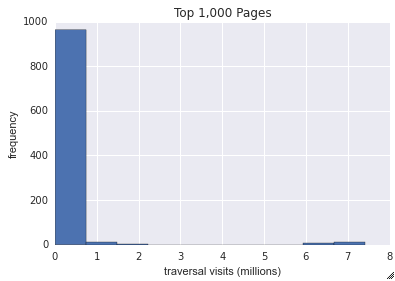
\includegraphics[width=\textwidth]{graphics/top_1k_pages.png}
    \end{subfigure}
    \begin{subfigure}[b]{0.4\textwidth}
        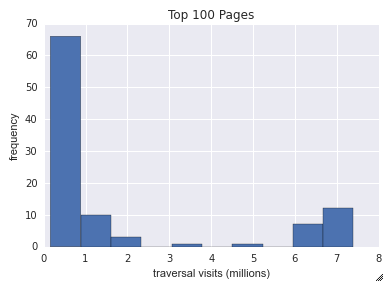
\includegraphics[width=\textwidth]{graphics/top_100_pages.png}
    \end{subfigure}
\end{figure}


\begin{figure}[H]
\centering
    \caption{highest ranking articles by number of traversals}
    \begin{subfigure}[b]{0.8\textwidth}
        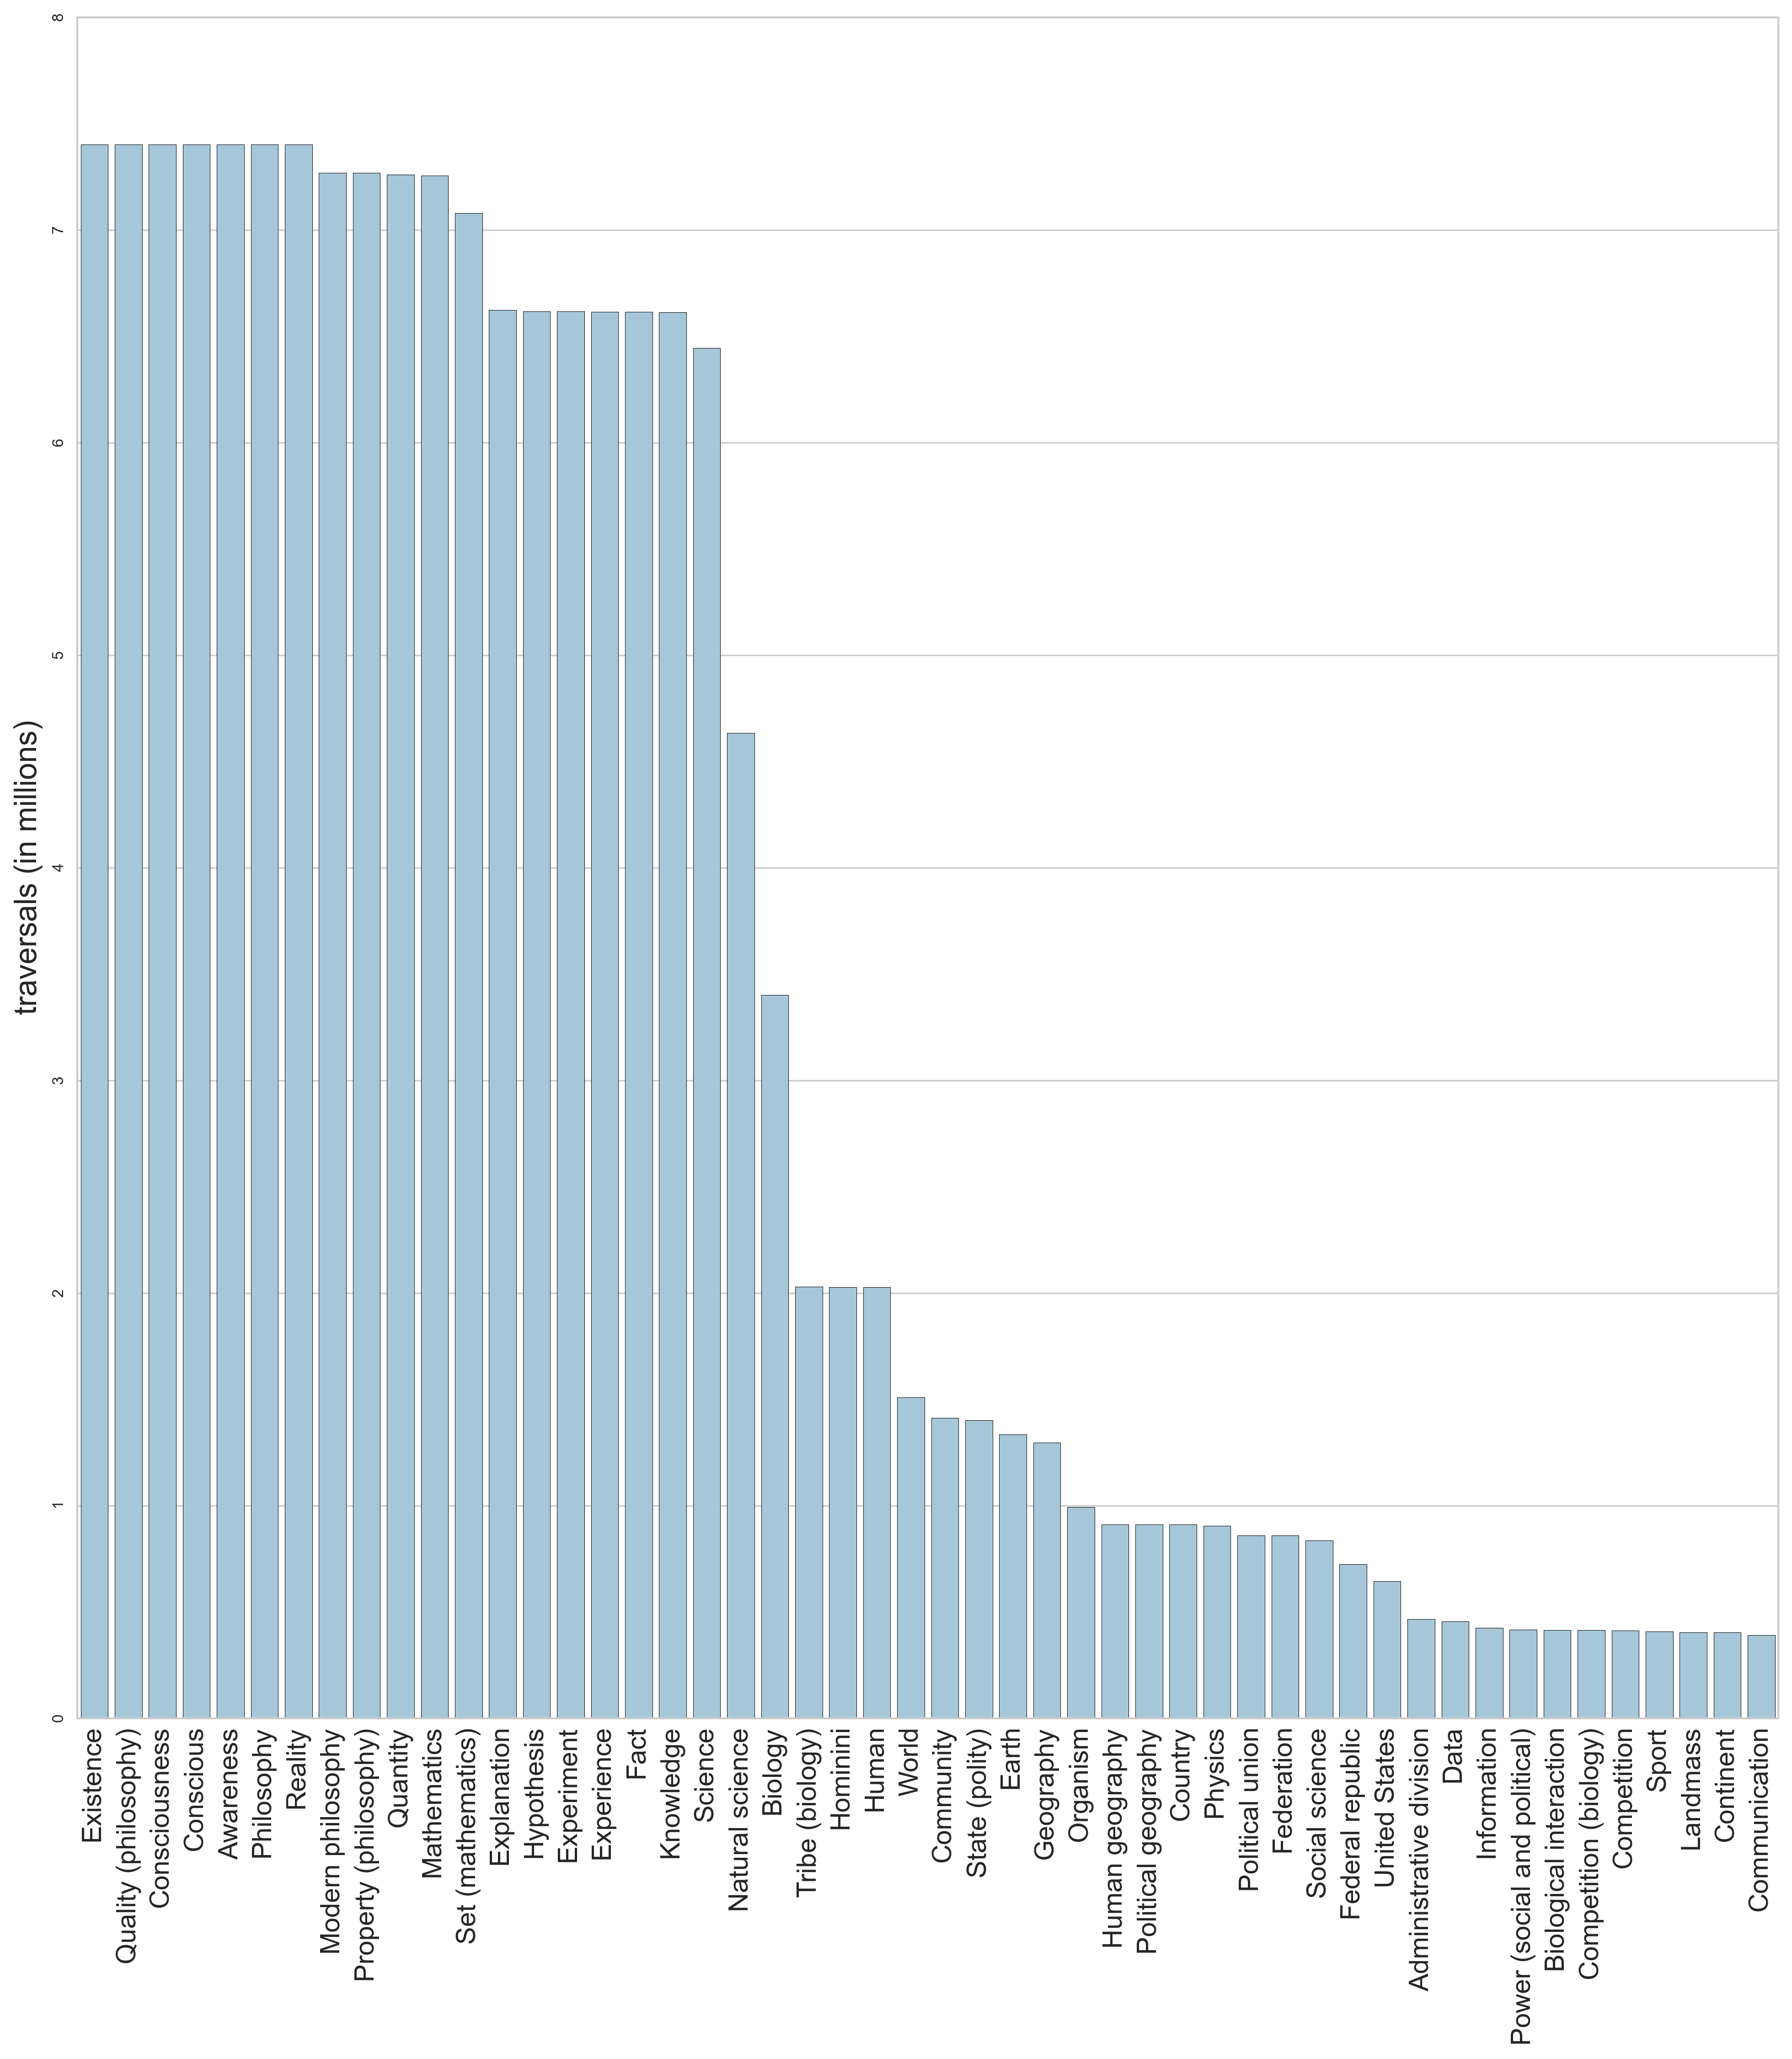
\includegraphics[width=\textwidth, angle=-90]{graphics/top_articles_list.png}
    \end{subfigure}
\end{figure}

The ranking by traversals reveals a cyclic structure marked by identical traversal numbers for the highest ranking 7 articles. By analyzing the traversal feeds, we can identify which articles in particular are the funnels or highest ranking within a particular cluster.

\red{\bt{TODO}}\\
\red{((look at other descriptives about a distribution or even descriptors of power-law))}\\


\subsection{Traversal Path Length}

By tracking the number of traversals to a repeated article or an invalid link, we can measure
the path length starting at any given article. 
We discovered the longest path length is 365, following 365 calendar days of Orthodox Liturgics, where the first link of today's Liturgic article links to the next day's and so on. Curiously, 
at on the last calendar day the article links back to the first day.
Similarly lengthy traversal paths included articles on the history of a nation on a particular year, for example 1953 in Scotland or 1560s in architecture.

Of the 11 million articles in our sample, 5.5 million had a path lenght of zero, meaning the first link is an invalid link or the article links to itslef (see section of cycles).
The most frequent path length is 29, with an interquartile range of (26, 30). The distribution of 
path lengths is similarly power-law like with few pages at the extreme of 355 traversals in their path length, while the majority is between 26-30.

\begin{figure}[H]
\centering
    \caption{Longest Path Lengths}
    \begin{subfigure}[b]{0.5\textwidth}
        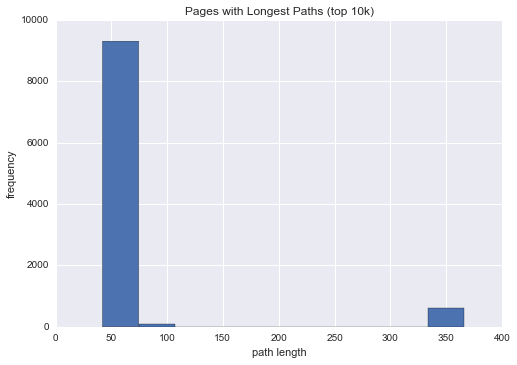
\includegraphics[width=\textwidth]{graphics/top_1k_path_length.png}
    \end{subfigure}
\end{figure}

\subsection{Basins of Attraction and Traversal Feeds}

A basin of attraction in our network is collection of path-connected articles. These articles do not necessarily form a loop, but may end at an invalid link. These basins are one way of measuring the center the of a network. If we rank the basins of attraction based on the accumulated number of ttraversals we find: many basins around philosophy: 

\begin{figure}[H]
\centering
    \caption{Longest Path Lengths}
    \begin{subfigure}[b]{0.5\textwidth}
        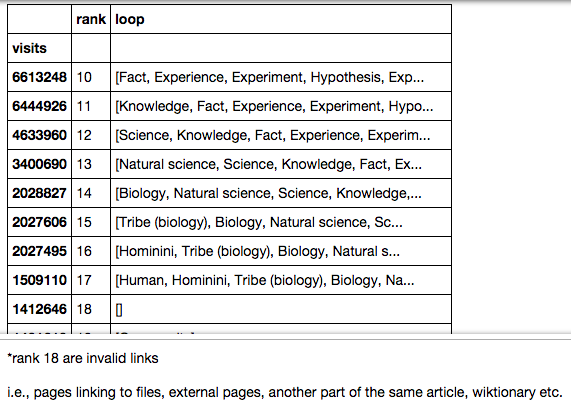
\includegraphics[width=\textwidth]{graphics/top_basins.png}
    \end{subfigure}
\end{figure}

Excluding any basins containing Philosophy, we find basins of attractions around Community, 
Landmass, Federal Government, Belief System, Presentation, and similarly foundational human concepts. This remarkable results confirms the foundational quality these ideas have in our english-based society. 
Whereby these concepts naturally arose out fo the links structure formed by teh owrk of many individuals working independtly on many topics often far aflied from one another. 
Curiously, gas and India both appear right after the foundational ideas, perhaps indicating the importance of these perhaps geographically or by population (second most populous country in the world) and gas which could refer to one fothe four fundamental states of matter or one of the most prized resources in the world.

\red{((maybe add graphic))}

Although identifying basins of attraction identifies a group of fundamental ideas, 
using the accumulated traversals, we can't identify whether one or more of the pages is a funnel. 
Among Philosophy, Existence, Knowledge, one page may be a funnel while the remaining simply happened to be connected to an article with many traversals. By measuring, where the traversal feeds, that is the number of traversals an article feeds into a loop, we can identify special funnel pages, 
which are part of a larger basin of attraction. Remarkable, within the Philosophy basin, 
Philosophy seems to be the singular funnel, accumulating an overwhelming majority of the traversals in the philosophy basin, with reality much farther behind (contributing a mere $.2\%$ of the 
traversals in the loop): 

\begin{figure}[H]
\centering
    \caption{Top Funnels}
    \begin{subfigure}[b]{0.5\textwidth}
        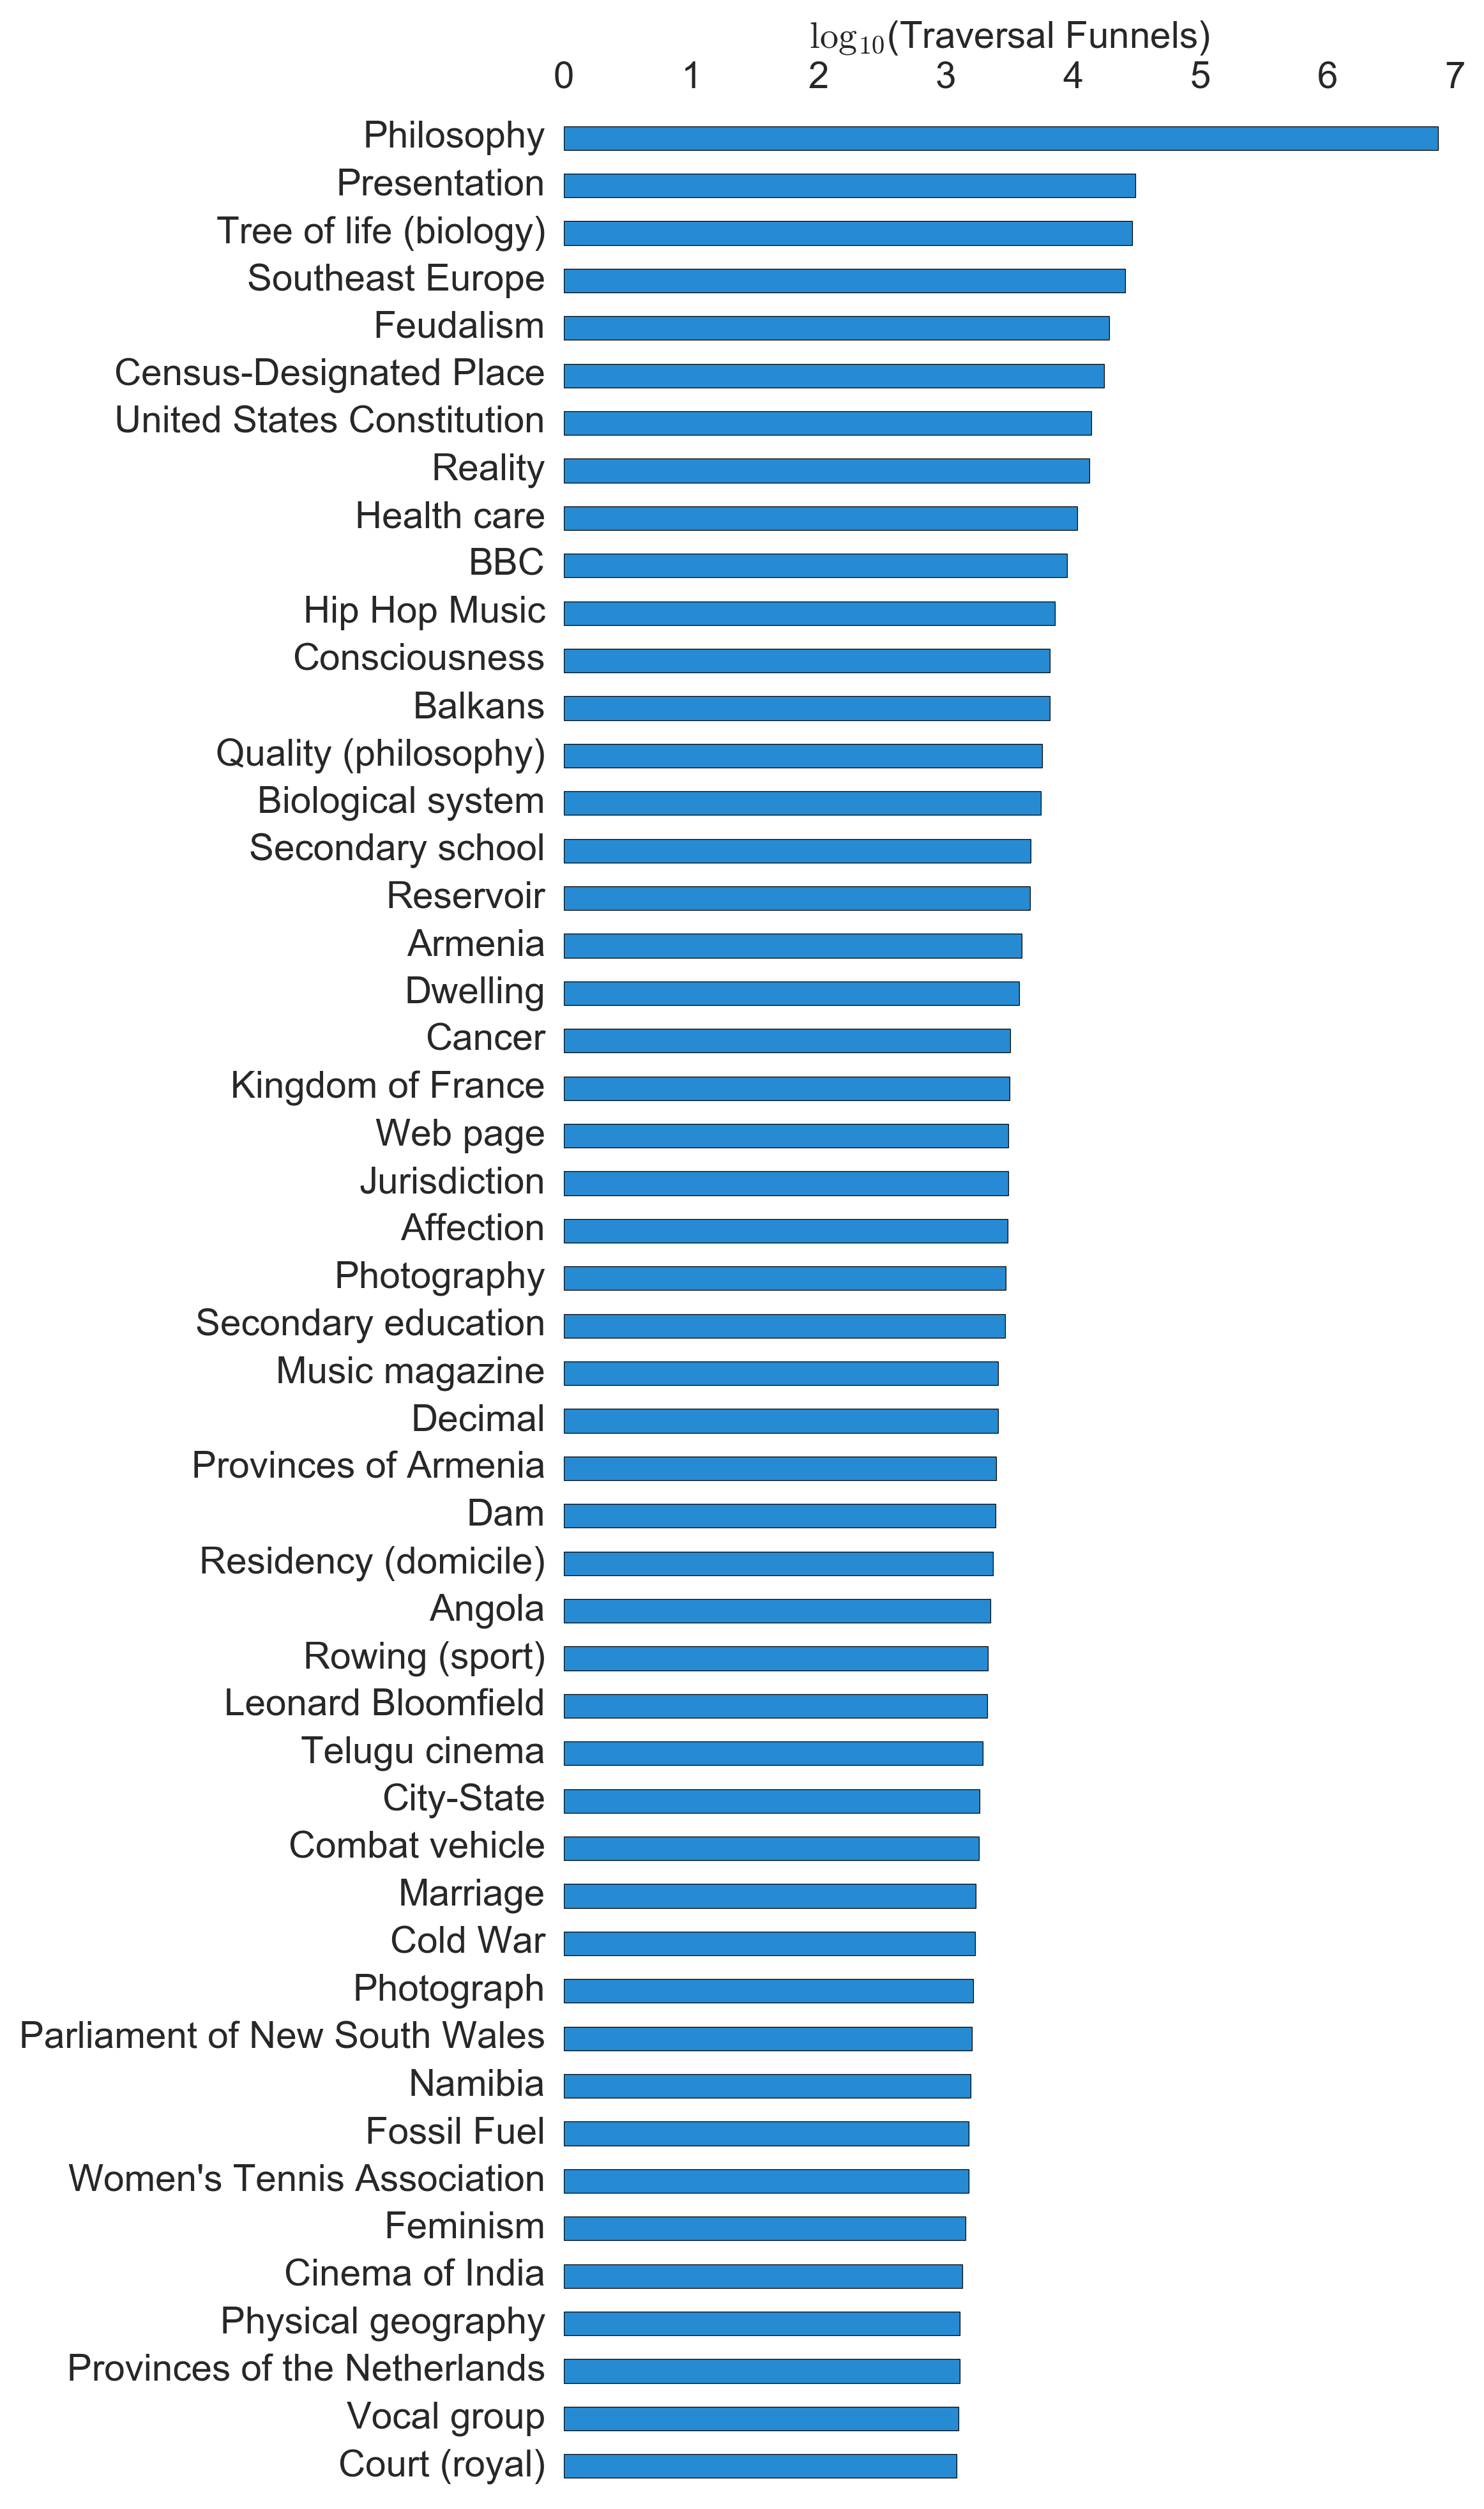
\includegraphics[width=\textwidth]{graphics/top_funnels.png}
    \end{subfigure}
\end{figure}


By measuring the number of traversals an article feeds into a loop, rather than measuring the accumulation, we measure how remarkable the traversals are around Philosophy. The second ranking page on teh list, Presentation, is dwarfed at a mere $.4\%$ of the traversal feeds Philosophy holds. 
Nonetheless, the list reveals a curious list of top pages including biology as the foundation of life, presentation a fundamental human act, as well as ideas of geographical and political import. Naturally, the page for Census-Designated Place makes an appearance on the top 10, as an accumulation place for the geographical regions in the US. Other topics of cultural and political importance today are Health Care (around which much political debate, science, and economics has been discussed), engaging a large number of our population ((cite something)). As well as Hip Hop or BBC, which are of cultural import. Other high ranking pages include historical events such as the Cold War, Fossil Fuel.

\subsection{Network Cycles}

By tracking traversals we can also measure true network cycles (loops) rather than a simple chain
of connected articles with a dead end. While many of the lengthy paths we discussed in an earlier section terminate at an invalid link, the Eastern Orthodox Liturgics do form a true cycle in the network with a lenght of 365, one article per calendar day looping back to the January first. Other, less lengthy cycles also exist with lengths between 60-75 traversals. These cycles include Historical pages, Judicial Pages such as the Legislative Assembly of Ontario and various Japanese eras dating back to the 8th or 9th centuries.


Since articles iwth a path-length of two yielded curious results, we also measured and ranked the top 2-cycles in the network by accumulated traversals: 

\begin{figure}[H]
\centering
\caption{highest ranking 2-Cycles}
    \begin{subfigure}[b]{0.8\textwidth}
        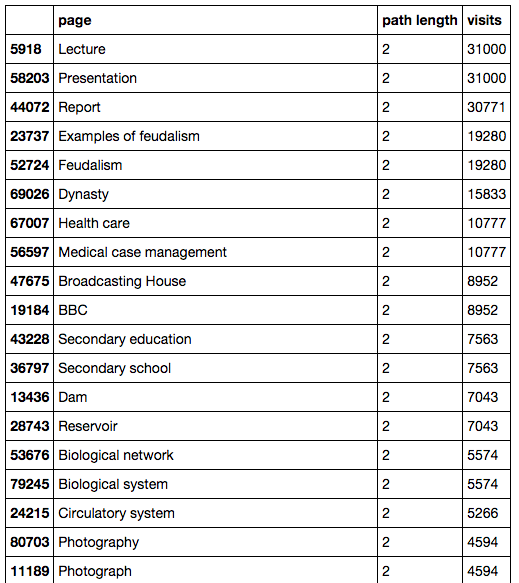
\includegraphics[width=\textwidth]{graphics/top_2loops.png}
    \end{subfigure}
\end{figure}

Of the 11 million artilces, only 83.6k are true 2-cycles. The average cycle traversals is 8, fewer than the typical article. However, Presentation does hold 31k traversals.

The top articles tended to be mere synoms rather than meaningful connections: Lecture and Presentation; Secondary eduaction adn seconday school; biological network and biological system; photogay and photograph. Outside the higest ranking articles, we does see a more meaningful connection among articles in 2-cycles: inventor to product: Voere -> VEC-91; book to author: Anatomy of Britain -> Anthony Sampson; event to organizer: Poetry Bus Tour -> Wave Books.

We also measured 3-cycles, cycles with length fewer than 100 etc. 3-Cycles were still expressing similar ideas or capturing synomous articles for similar ideas: Tree of life (biology) -> Tree of life (disambiguation) and Tree of life. Similarly with Cinema of India, Indian Cinemay and Telugu cinema  There were 74K 3-cycles. Once we looked beyond cycles of lenght 10 however, philosophy seemed to dominate along with the remaining list of higest ranking articles--this confirms the typical path length for high ranking pages is typically less than 10.

\begin{figure}[H]
\centering
\caption{highest ranking 3-Cycles}
    \begin{subfigure}[b]{0.8\textwidth}
        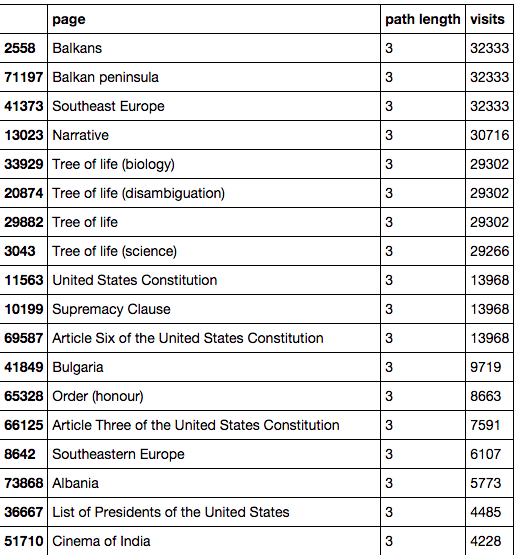
\includegraphics[width=\textwidth]{graphics/top_3loops.png}
    \end{subfigure}
\end{figure}
\newpage
\section*{Style Guide}

\begin{itemize}
\item Web Terms
    \begin{itemize}
        \item \bt{article} instead of page
        \item \bt{invalid link} (instead of dead or bad link)
    \end{itemize}
\item Measurements
    \begin{itemize}
        \item \bt{traversals} = node weight
        \item \bt{path length} = number of articles traversed until an invalid link or a repeated article
        \item \bt{traversal feeds} = traversals before a cycle is reached.
    \end{itemize}
\item Network Properties
    \begin{itemize}
        \item \bt{cycle} (permutation from abstract algebra) instead of loop
        \item \bt{path-connected articles} for both cycles and articles along the same path leading to an 
    invalid link
        \item \bt{basin of attraction} a path-connected group of articles (not necessarily at loop) with a high ranking number of traversals.
    \end{itemize}
\end{itemize}



\end{document}
